% ------------------------------------------------------------------------
%  Instituto Mauá de Tecnologia
%  Núcleo de Sistemas Eletrônicos Embarcados - NSEE
%   Rodrigo Romano & Rafael Corsi
% 					 corsiferrao@gmail.com
%  		
%  Projeto CITAR
%	Meta 4
% 	Especificação do produto
% 	Acionamento motor BLDC para rodas de reação
%
%	Junho de 2014
% ------------------------------------------------------------------------
% ------------------------------------------------------------------------
% Modelo criado por: Rodrigo Romano
% "Rafael Corsi" <corsiferrao@gmail.com>
% ------------------------------------------------------------------------

%\documentclass[12pt,a4paper,twoside=semi, headinclude]{scrreprt}
\documentclass[
    fontsize=12pt,          % fontsize
    paper=a4,               % page size a4
    firsthead=on,           % display header on first page
    firstfoot=on,           % display footer on first page
    pagenumber=off,         % position of the page number
    parskip=half,           % Use indent instead of skip, half, false
    enlargefirstpage=on,    % more space on first page
    fromalign=left,         % placement of name in letter head
    fromrule=afteraddress,  % separate the address with a line in letter head, false or aftername
    fromemail=off,          % turn on email of sender
    fromurl=off,            % print URL of sender
    fromphone=off,          % turn on phone of sender
    fromlogo=off,           % turn on logo of sender
    addrfield=on,           % address field for envelope with window, on or true
    subject=titled,         % placement of subject, beforeopening or titled
    foldmarks=off,          % print foldmarks
    numericaldate=off,      % display date in numbers only
    KOMAold]{scrreprt}
%\usepackage[a4paper,left=3.5cm,right=1.5cm,top=3cm,bottom=2.5cm]{geometry}

\usepackage[utf8]{inputenc}       %Permite acentuação
\usepackage[T1]{fontenc}
\usepackage[english,brazil,brazilian]{babel}
\usepackage[centertags]{amsmath}



% ------------------------------------------------------------------------
\usepackage[automark,headsepline]{scrlayer-scrpage}
%\clearpairofpagestyles
\cfoot[\pagemark]{\pagemark}
\lehead{\headmark}
\rohead{\headmark}
\cfoot[\raisebox{-0.5em}{ -- \, \textnormal{\thepage} \, --}]{\raisebox{-0.5em}{ -- \, \textnormal{\thepage} \, --}}
\pagestyle{scrheadings}
%\include{authorpart}
% ------------------------------------------------------------------------

\usepackage{lmodern,
			url,
			hyperref,
			multirow,
			array,
			indentfirst,
			ncccomma,
			pst-node,
			pstricks,
			schemabloc,
			amssymb,
			amsfonts,
			graphicx,
			etoolbox, 
			pdfpages,
			hyperref,
			paralist,
			tabularx,
			pdflscape,
			color,				
			doc,
			vhistory,
			tcolorbox,
			titlepic,
			hyperref}
			
\usepackage[titletoc,toc,title]{appendix}
% ------------------------------------------------------------------------
% Reduz espacamento na bibliografia
%\usepackage{natbib}
%\setlength{\bibsep}{0.0pt}

%Matem figura na secção !
%\usepackage[section]{placeins}

% sub figuras
%ajuste do tamanho entre figuras
\usepackage{subfigure}
\setlength\subfigcapmargin{0.8em}

% Fuzz 
\hfuzz1pt % Don't bother to report over-full boxes if over-edge is < 2pt

% Numeração das notas de rodapé 
\renewcommand{\thefootnote}{\fnsymbol{footnote}}

% Different font in captions 
\newcommand{\captionfonts}{\small}

\makeatletter  % Allow the use of @ in command names
\long\def\@makecaption#1#2{%
  \vskip\abovecaptionskip
  \sbox\@tempboxa{{\captionfonts #1: #2}}%
  \ifdim \wd\@tempboxa >\hsize
    {\captionfonts #1: #2\par}
  \else
    \hbox to\hsize{\hfil\box\@tempboxa\hfil}%
  \fi
  \vskip\belowcaptionskip}
\makeatother   % Cancel the effect of \makeatletter

% Espaçamento
\setlength{\parindent}{30pt} \setlength{\parskip}{6pt}
\newlength{\defbaselineskip}
\setlength{\defbaselineskip}{\baselineskip}

\newcommand{\setlinespacing}[1]{\setlength{\baselineskip}{#1 \defbaselineskip}}
% ---
\newcommand{\PreserveBackslash}[1]{\let\temp=\\#1\let\\=\temp}
\let\PBS=\PreserveBackslash %
\def\baselinestretch{1}
\setlinespacing{1.5}
% ------------------------------------------------------------------------
% Use the microtype package for better typography
% http://www.khirevich.com/latex/microtype/
%
% activate={true,nocompatibility} - activate protrusion and expansion
% final - enable microtype; use "draft" to disable
% tracking=true, kerning=true, spacing=true - activate these techniques
% factor=1100 - add 10% to the protrusion amount (default is 1000)
% stretch=10, shrink=10 - reduce stretchability/shrinkability (default is 20/20)
\usepackage[activate={true,nocompatibility},
			final,
			tracking=true,
			kerning=true,
			spacing=true,
			factor=1100,
			stretch=10,
			shrink=10]
			{microtype} 

% Possibilita que caracteres saiam da margem p/ melhor caber o texto
\SetProtrusion{encoding={*},
			   family={bch},
			   series={*},size={6,7}}
               {1={ ,750},2={ ,500},3={ ,500},4={ ,500},5={ ,500},
               6={ ,500},7={ ,600},8={ ,500},9={ ,500},0={ ,500}}

\microtypecontext{spacing=nonfrench}
% ------------------------------------------------------------------------
               
% Todo notes
%\usepackage[disable]{todonotes}
\usepackage[colorinlistoftodos]{todonotes}  
\setlength{\marginparwidth}{2cm}
\reversemarginpar             
%\makeatletter\let\chapter\@undefined\makeatother

\newcommand\todoin[2][]{\todo[inline, caption={2do}, #1, color={red!100!green!33}]{
\begin{minipage}{\textwidth-4pt}#2\end{minipage}}}

% ------------------------------------------------------------------------

% Restora contagem da nota a cada pagina
\usepackage{perpage}
\MakePerPage{footnote}

% Qualidade e compressão do pdf
%\pdfminorversion=5
%\pdfcompresslevel=9
%\pdfobjcompresslevel=2

% ------------------------------------------------------------------------
% Possibilita inserir pdf com texto fora do arquivo
% util para figs geradas no inkscape
\newcommand{\executeiffilenewer}[3]{%
\ifnum\pdfstrcmp{\pdffilemoddate{#1}}%
{\pdffilemoddate{#2}}>0%
{\immediate\write18{#3}}\fi%
}

\newcommand{\includesvg}[1]{%
\executeiffilenewer{#1.svg}{#1.pdf}%
{inkscape -z -D --file=./Figs/#1.svg %
--export-pdf=./Figs/#1.pdf --export-latex}%
\input{./figs/#1.pdf_tex}%
}
\usepackage{natbib}
%------------------------------------------------------------------------	
\usepackage{tikz}
\graphicspath{ {./figs/} }
% ------------------------------------------------------------------------
\newtcolorbox[auto counter,number within=section]{TBD-BOX}[2][]{%
colback=red!5!white,colframe=darkgray,fonttitle=\bfseries,
title=TBD.~\thetcbcounter: #2,#1}
% ------------------------------------------------------------------------
% http://latexcolor.com/
% cores dos todos
\definecolor{TBC}{rgb}{0.98, 0.91, 0.71}  	%bananamania
\definecolor{Corsi}{rgb}{0.53, 0.66, 0.42}  %
%\definecolor{TBC2}{rgb}{1.0, 0.71, 0.76} 		%lightpink
\definecolor{TBC2}{rgb}{0.86, 0.82, 1.0} %lightmauve
\definecolor{darkgray}{rgb}{0.66, 0.66, 0.66}
\definecolor{aliceblue}{rgb}{0.94, 0.97, 1.0}
% ------------------------------------------------------------------------

\title		{   \LARGE
				Instituto Mauá de Tecnologia \\
				Núcleo de Sistemas Eletrônicos Embarcados - NSEE \\ 
				\vspace{10px}
				\huge
				Especificação do Produto \\
				SpaceWire Data Feed \\
			}
\author		{
				 Rafael Corsi \\ \small 	
				\href{mailto:rafael.corsi@maua.com}{rafael.corsi@maua.com}
			}
%\subject	{Núcleo de Sistemas Eletrônicos Embarcados - NSEE}			
\titlepic	{
\includegraphics[width=0.4\textwidth]{maua_logo}}
%\lowertitleback{}

% ------------------------------------------------------------------------
\begin{document}
% ------------------------------------------------------------------------
\maketitle
\tableofcontents
% ------------------------------------------------------------------------
%%---------- Revisão
\begin{versionhistory}
  \vhEntry{0.0.1}{24.6.14}{Corsi}{Criação do documento}
\end{versionhistory}
% ------------------------------------------------------------------------
%%---------- Lista de distribuição
%\section*{Lista de distribuição}
%\todo[inline]{inserir emails}
%\begin{itemize}
%	\item IMT	
%	\begin{itemize}
%		\item Rafael Corsi Ferrão 
%		\item Rodrigo A. Romano 
%		\item Sergio Ribeiro Augusto 
%		\item Vanderlei Cunha Parro
%		\item José Carlos 
%		\item Magda 
%		\item Raphael Ballet
%	\end{itemize}
%	\item INPE
%	\begin{itemize}
%		\item Silvio ?
%	\end{itemize}
%	\item Externo
%	\begin{itemize}
%		\item Saulo
%	\end{itemize}	
%\end{itemize}

% ------------------------------------------------------------------------
% -----------------
\chapter{Introdução}


% -----------------
\section{Finalidade}

O projeto proposta chamado de SpW-Data-Feed é um exemplo de aplicação do protocolo SpaceWire, a ser usado na bancada de experimento do projeto CITAR. 

% -----------------
\section{Escopo Geral}

Definição das especificações gerais do projeto e propostas de implementação.

% -----------------
\section{Referências}


\todo[inline, color=Corsi]{listar documentos de input - IMT e CITAR}

% -----------------
\section{Visão Geral}

O objetivo do projeto é desenvolver um hardware de uso de bancada capaz de ler e escrever em conversores A/D e D/A e em saídas e entradas digitais. O dispositivo será conectado em um nó SpaceWire com as configurações e dados trafegando sob o protocolo RMAP.

O projeto está sendo desenvolvido no âmbito do projeto de Circuitos Integrados Tolerantes a Radiação (CITAR), coordenado pelo pesquisador Saulo Finco do Centro de Tecnologia da Informação Renato Archer (CTI). 


% -----------------
\section{Equipe}

\begin{itemize}
	\item Profissionais do IMT:
	\begin{itemize}
		 \item Rafael Corsi Ferrão (coordenação)
	\end{itemize}
	
	\item Bolsistas:
	\begin{itemize}
		\item IC Dennis Teles (execução)
	\end{itemize}
\end{itemize}


\chapter{Posicionamento}

% ----------------------------------------------------------------
\section{Descrição Geral do Projeto}

Desenvolver um dispositivo embarcado (SpWDataFeed) em uma FPGA capaz de realizar a leitura de conversores A/D, escrever em conversores D/A, acionar e ler entradas digitais. Esse dispositivo será conectado em uma rede SpaceWire com o protocolo RMAP.

O SpWDataFeed será utilizado para demonstrar os benefícios do protocolo SpW em uma aplicação similar ao encontrado em satélites.

% ----------------
\section{Representação Gráfica do Produto}

A arquitetura proposta para a implementação do SpWDataFeed é ilustrado na Fig. \ref{fig:arch}, onde o acesso ao dispositivo é feito via comandos RMAP. Uma interface seria RS232 é utilizada para configuração e debug do dispositivo. 

O módulo implementa leitura de conversores A/D (SpI, I2C, paralelo (\textbf{TBD})) através do A/D Módulo, escrita em conversores D/A (\textbf{TBD}) pelo D/A módulo e acesso direto a I/Os digitais via os módulos Din e Dout.

\begin{figure}[ht!]
	\centering
	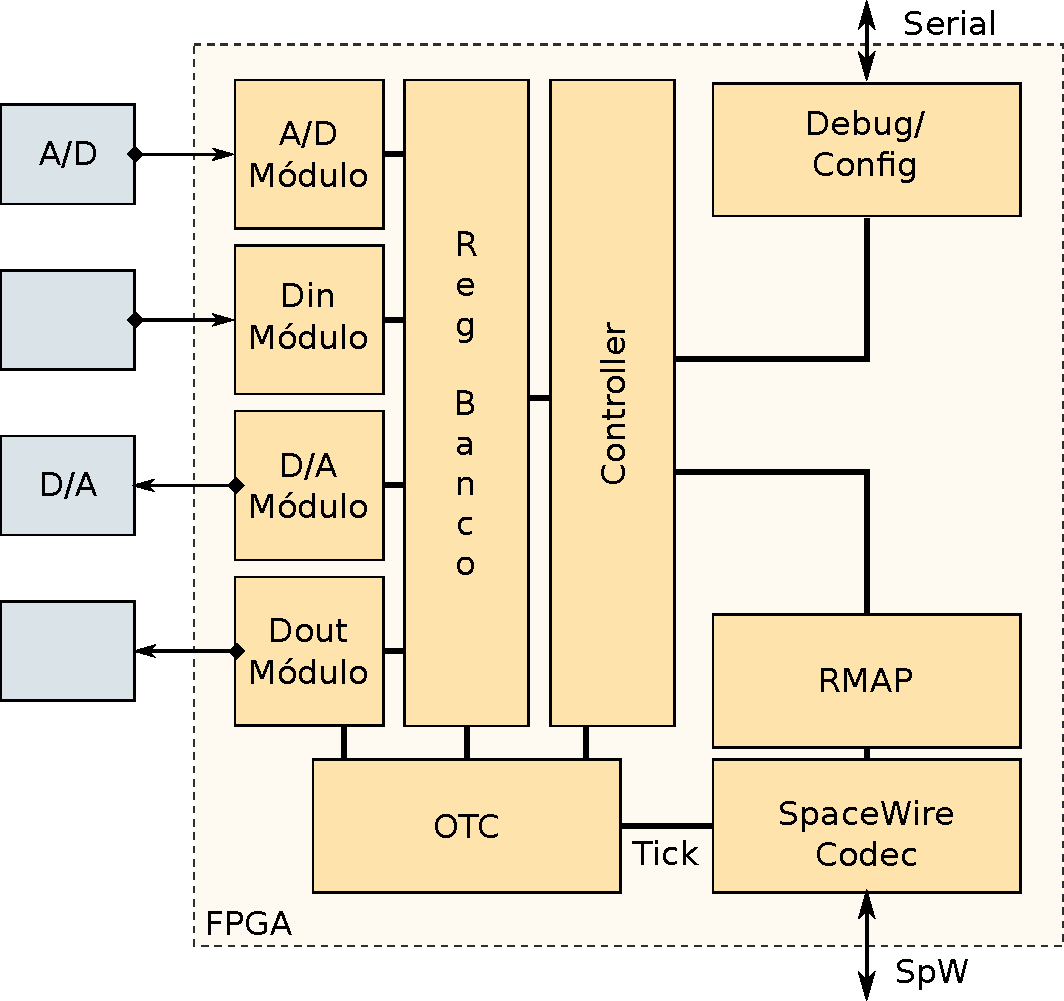
\includegraphics[width=0.8\linewidth]{./figs/arch}
	\caption{Diagrama de blocos}
	\label{fig:arch}
\end{figure}

A arquitetura é concebida de forma que o dispositivo possa ser utilizado para controle e acionamento de diversos sistemas aerospaciais, tais como: abertura de painel solar, controle de experimento.

\chapter{Identificação dos Componentes Envolvidos e Responsáveis}

\section{SpaceWire Codec}

IP core que implementa o protocolo SpaceWire, pretende-se utilizar o codec desenvolvido no projeto CITAR mas existem outras opções, tais como :

\begin{itemize}
	\item SpaceWire NSEE
	\item SpaceWire Light
	\item SpaceWire CEA
\end{itemize}

\section{RMAP}

O protocolo RMAP será a forma de acesso e controle da aplicação, via comandos de escrita, será possível configurar os modos de operação assim como escrever nos conversores D/A e saídas digitais. Comandos de leitura serão utilizados para acesso assíncrono ao dados dos conversores A/D e portas digitais de entrada. Comandos de escrita da aplicação para o nó remoto, será utilizado para envio periódico das informações desses sensores.

Estudar viabilidade de uso do código já implementado para o Simucam. O comando de Read-Write não é implementado nesse core.

\section{OTC - On Board Time Controller}

O OTC será o responsável pela gestão dos sinais de sincronismo internos assim como o fornecedor de timestamp para o envio junto com os dados. Esse bloco é sincronizado com o restante dos nós via comandos de timecode enviados no canal SpW.

\section{Controller}

Core responsável por implementar a máquina de estados que controla a aplicação. Estudar a possibilidade de embarcar um uP.

\section{Reg. Banco}

Banco de registros compartilhado entre os módulos, para armazenamento de dados e configurações.

\section{Módulo A/D}

Módulo responsável pelo controle dos conversores A/D e escrita dos dados no Reg. Banco.

\section{Módulo D/A}

Módulo responsável pelo controle dos conversores D/A com os parâmetros configurados no Reg. Banco.

\section{Módulo Din}

Módulo responsável pelo controle das entradas digitais e escrita dos dados no Reg. Banco.

\section{Módulo Dout}	

Módulo responsável pelo controle das saídas digitais com os parâmetros configurados no Reg. Banco.

\section{Comandos}


\subsection{Definir zona de memória}

% ----------------
\chapter{Recursos do Produto}

\section{Fases do projeto}

\begin{enumerate}
	\item Especificação detalhada
	\item Implementação
	\item Teste 
\end{enumerate}

\section{Ferramentas}

Para implementação inicial, pretende-se utilizar a placa de desenvolvimento GR-PCI-XC5V da pender que possui uma FPGA Xilinx Virtex 5. O desenvolvimento será feito no software ISE com simulações tanto no ISIM quanto no ModelSim.

Para testes a nível SpW, utilizar o USB Brick da StarDundee.

\section{Gestão}



% ----------------
	\apptocmd{\thebibliography}{\footnotesize}{}{}
	\bibliographystyle{unsrt}
	\addcontentsline{toc}{section}{Referências Bibliográficas}
	\bibliography{bibliografia}

%-----------------------------------------------------
\end{document}
% ------------------------------------------------------------------------

% ------------------------------------------------------------------------
% COLAS
% ------------------------------------------------------------------------

% ------------------------------------------------------------------------
%\begin{figure}[ht!]  
%	\centering
%		\includegraphics[width=0.6 \columnwidth,angle=0]{figs/svpwm.pdf}
%	\caption{Acionamento SVPWM}
%	\label{fig:svpwm}
%\end{figure}
% ------------------------------------------------------------------------

% ------------------------------------------------------------------------
%\begin{tcolorbox}[title=Objetivo central]
%	Desenvolver um dispositivo embarcado em uma FPGA capaz de realizar tanto o acionamento como o controle de motores de corrente contínua sem escovas (BLDC)
%\end{tcolorbox}
% ------------------------------------------------------------------------
%\begin{TBD-BOX}[label={myautocounter}]{Metodologia}
%	\begin{itemize}
%		\item Verificar especificação com CITAR
%		\item TestBenchs
%	\end{itemize}
	%\end{TBD-BOX}